% !TeX spellcheck = en_GB
% \begin{figure}[h!]
% 	\centering
% 		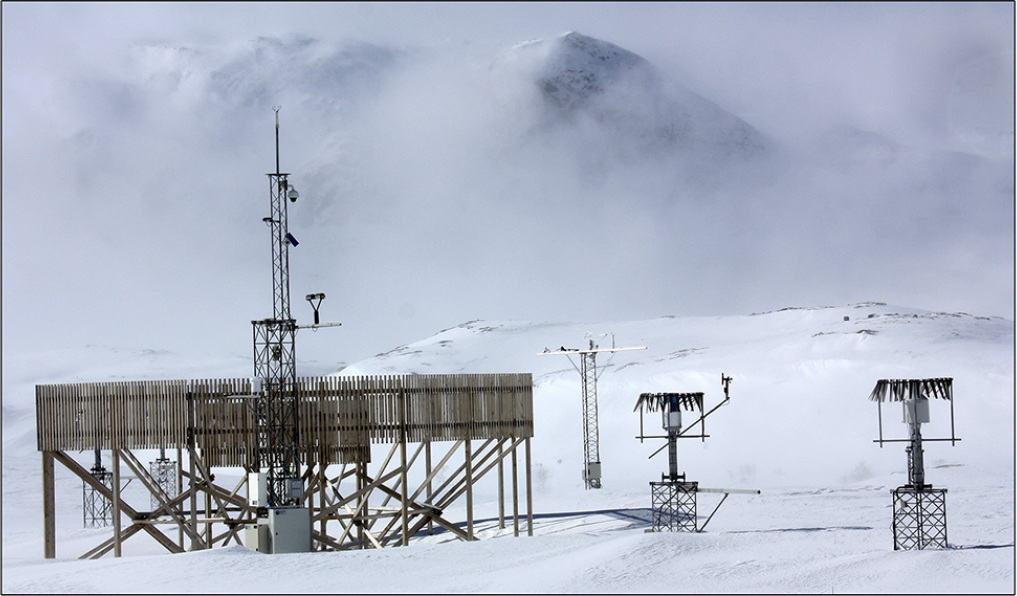
\includegraphics[width=0.55\textwidth]{./fig_instruments/Dofe.png}
% 	\caption{Picture, showing the double fence and unprotected precipitation gauges at the measurement site Haukeliseter. Picture taken from \cite{wolff_derivation_2015}.}\label{fig:Dofe}
% \end{figure}

\begin{wrapfigure}[10]{r}{0.44\textwidth}
	\vspace{-\normalbaselineskip}
	\centering
	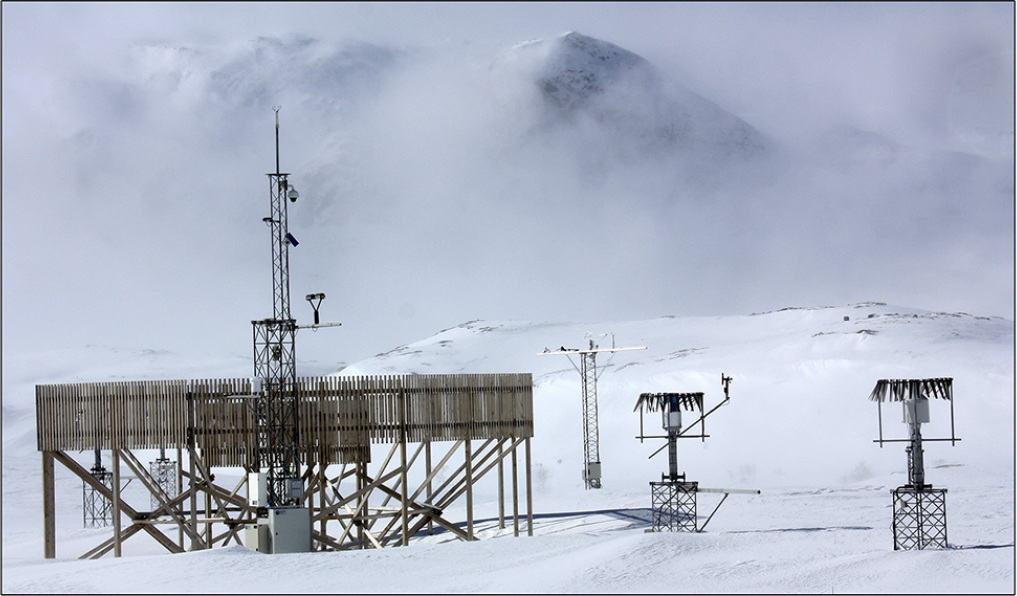
\includegraphics[width=0.4\textwidth]{./fig_instruments/Dofe.png}
	%	\vspace{-10pt}
	\caption{Double fence and unprotected precipitation gauges at Haukeliseter, from \cite{wolff_derivation_2015}. The prevailing wind from east comes from the left side in the image. }\label{fig:Dofe}
	\vspace{-\normalbaselineskip}
\end{wrapfigure}
